%%%%%%%%%%%%%%%%%%%%%%%%%%%%% Define Article %%%%%%%%%%%%%%%%%%%%%%%%%%%%%%%%%%
\documentclass{article}
%%%%%%%%%%%%%%%%%%%%%%%%%%%%%%%%%%%%%%%%%%%%%%%%%%%%%%%%%%%%%%%%%%%%%%%%%%%%%%%

%%%%%%%%%%%%%%%%%%%%%%%%%%%%% Using Packages %%%%%%%%%%%%%%%%%%%%%%%%%%%%%%%%%%
\usepackage{geometry}
\usepackage{graphicx}
\usepackage{amssymb}
\usepackage{amsmath}
\usepackage{amsthm}
\usepackage{empheq}
\usepackage{mdframed}
\usepackage{booktabs}
\usepackage{lipsum}
\usepackage{graphicx}
\usepackage{color}
\usepackage{psfrag}
\usepackage{pgfplots}
\usepackage{bm}
%%%%%%%%%%%%%%%%%%%%%%%%%%%%%%%%%%%%%%%%%%%%%%%%%%%%%%%%%%%%%%%%%%%%%%%%%%%%%%%

% Other Settings

%%%%%%%%%%%%%%%%%%%%%%%%%% Page Setting %%%%%%%%%%%%%%%%%%%%%%%%%%%%%%%%%%%%%%%
\geometry{a4paper}

%%%%%%%%%%%%%%%%%%%%%%%%%% Define some useful colors %%%%%%%%%%%%%%%%%%%%%%%%%%
\definecolor{ocre}{RGB}{243,102,25}
\definecolor{mygray}{RGB}{243,243,244}
\definecolor{deepGreen}{RGB}{26,111,0}
\definecolor{shallowGreen}{RGB}{235,255,255}
\definecolor{deepBlue}{RGB}{61,124,222}
\definecolor{shallowBlue}{RGB}{235,249,255}
%%%%%%%%%%%%%%%%%%%%%%%%%%%%%%%%%%%%%%%%%%%%%%%%%%%%%%%%%%%%%%%%%%%%%%%%%%%%%%%

%%%%%%%%%%%%%%%%%%%%%%%%%% Define an orangebox command %%%%%%%%%%%%%%%%%%%%%%%%
\newcommand\orangebox[1]{\fcolorbox{ocre}{mygray}{\hspace{1em}#1\hspace{1em}}}
%%%%%%%%%%%%%%%%%%%%%%%%%%%%%%%%%%%%%%%%%%%%%%%%%%%%%%%%%%%%%%%%%%%%%%%%%%%%%%%

%%%%%%%%%%%%%%%%%%%%%%%%%%%% English Environments %%%%%%%%%%%%%%%%%%%%%%%%%%%%%
\newtheoremstyle{mytheoremstyle}{3pt}{3pt}{\normalfont}{0cm}{\rmfamily\bfseries}{}{1em}{{\color{black}\thmname{#1}~\thmnumber{#2}}\thmnote{\,--\,#3}}
\newtheoremstyle{myproblemstyle}{3pt}{3pt}{\normalfont}{0cm}{\rmfamily\bfseries}{}{1em}{{\color{black}\thmname{#1}~\thmnumber{#2}}\thmnote{\,--\,#3}}
\theoremstyle{mytheoremstyle}
\newmdtheoremenv[linewidth=1pt,backgroundcolor=shallowGreen,linecolor=deepGreen,leftmargin=0pt,innerleftmargin=20pt,innerrightmargin=20pt,]{theorem}{Theorem}[section]
\theoremstyle{mytheoremstyle}
\newmdtheoremenv[linewidth=1pt,backgroundcolor=shallowBlue,linecolor=deepBlue,leftmargin=0pt,innerleftmargin=20pt,innerrightmargin=20pt,]{definition}{Definition}[section]
\theoremstyle{myproblemstyle}
\newmdtheoremenv[linecolor=black,leftmargin=0pt,innerleftmargin=10pt,innerrightmargin=10pt,]{problem}{Problem}[section]
%%%%%%%%%%%%%%%%%%%%%%%%%%%%%%%%%%%%%%%%%%%%%%%%%%%%%%%%%%%%%%%%%%%%%%%%%%%%%%%

%%%%%%%%%%%%%%%%%%%%%%%%%%%%%%% Plotting Settings %%%%%%%%%%%%%%%%%%%%%%%%%%%%%
\usepgfplotslibrary{colorbrewer}
\pgfplotsset{width=8cm,compat=1.9}
%%%%%%%%%%%%%%%%%%%%%%%%%%%%%%%%%%%%%%%%%%%%%%%%%%%%%%%%%%%%%%%%%%%%%%%%%%%%%%%

%%%%%%%%%%%%%%%%%%%%%%%%%%%%%%% Title & Author %%%%%%%%%%%%%%%%%%%%%%%%%%%%%%%%
\title{Differential Equations}
\author{Patrick Chen}
%%%%%%%%%%%%%%%%%%%%%%%%%%%%%%%%%%%%%%%%%%%%%%%%%%%%%%%%%%%%%%%%%%%%%%%%%%%%%%%

\begin{document}
    \maketitle
    An ordinary differential equations (ODE) is a type of differential equation
    (DE) that contain derivatives with respect to only a single independent
    variable. It is called ordinary because it only contains one independent
    variable. The order of an ODE the highest derivative in the differential
    equation. The solution for a differential equation is a function that
    satisfies the differential equation on some interval. The solution may or
    may not be unique. An autonomous differential equation is a differential
    equation that has no explicit terms containing the independent variable.

    \section*{Shape of Differential Equation Graphs}
    It is possible to determine properties of the shape of a differential
    equation by examining the equation.
    \subsection*{Example}
    \[
        y'=x(y-1)^2
    \]
    When this differential equation is evaluated at a point $(x,y)$, the
    solution to the differential equation passing through the point $(x,y)$ must
    be the slope found.
    \begin{center}
        \begin{tabular}[c]{l|l l l}
            y x& -1 & 0 & 1 \\
            \hline
            1  & 0 & 0 & 0 \\
            0  & -1 & 0 & 1 \\
            -1 & -4 & 0 & 4 \\
        \end{tabular}
    \end{center}
    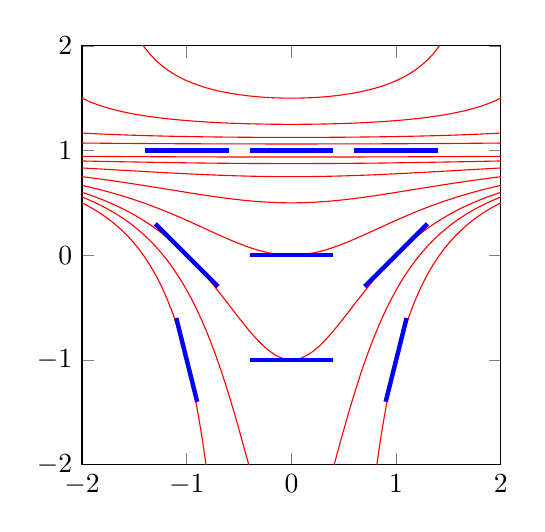
\begin{tikzpicture}
        \begin{axis}[
            axis equal image,
            xmin=-2,
            xmax=2,
            ymin=-2,
            ymax=2
            ]
             \addplot [
                domain=-2:2,
                samples=70,
                color=red
                ]
                {(-2*16+x^2-2)/(-2*16+x^2)};
             \addplot [
                domain=-2:2,
                samples=70,
                color=red
                ]
                {(-2*8+x^2-2)/(-2*8+x^2)};
             \addplot [
                domain=-2:2,
                samples=70,
                color=red
                ]
                {(-2*4+x^2-2)/(-2*4+x^2)};
             \addplot [
                domain=-1.9:1.9,
                samples=70,
                color=red
                ]
                {(-2*2+x^2-2)/(-2*2+x^2)};
             \addplot [
                domain=-2:-0.4,
                samples=70,
                color=red
                ]
                {(2*0+x^2-2)/(2*0+x^2)};
             \addplot [
                domain=0.4:2,
                samples=70,
                color=red
                ]
                {(2*0+x^2-2)/(2*0+x^2)};
             \addplot [
                domain=-2:2,
                samples=70,
                color=red
                ]
                {(2*0.25+x^2-2)/(2*0.25+x^2)};
             \addplot [
                domain=-2:2,
                samples=70,
                color=red
                ]
                {(2*0.5+x^2-2)/(2*0.5+x^2)};
             \addplot [
                domain=-2:2,
                samples=70,
                color=red
                ]
                {(2*1+x^2-2)/(2*1+x^2)};
             \addplot [
                domain=-2:2,
                samples=70,
                color=red
                ]
                {(2*2+x^2-2)/(2*2+x^2)};
             \addplot [
                domain=-2:2,
                samples=70,
                color=red
                ]
                {(2*4+x^2-2)/(2*4+x^2)};
             \addplot [
                domain=-2:2,
                samples=70,
                color=red
                ]
                {(2*8+x^2-2)/(2*8+x^2)};
             \addplot [
                domain=-2:2,
                samples=70,
                color=red
                ]
                {(2*16+x^2-2)/(2*16+x^2)};
             \addplot [
                domain=-1.4:-0.6,
                samples=70,
                color=blue,
                ultra thick
                ]
                {1};
             \addplot [
                domain=-1.3:-0.7,
                samples=70,
                color=blue,
                ultra thick
                ]
                {-(x+1)};
             \addplot [
                domain=-1.1:-0.9,
                samples=70,
                color=blue,
                ultra thick
                ]
                {-4*(x+1)-1};
             \addplot [
                domain=-0.4:0.4,
                samples=70,
                color=blue,
                ultra thick
                ]
                {1};
             \addplot [
                domain=-0.4:0.4,
                samples=70,
                color=blue,
                ultra thick
                ]
                {0};
             \addplot [
                domain=-0.4:0.4,
                samples=70,
                color=blue,
                ultra thick
                ]
                {-1};
             \addplot [
                domain=0.6:1.4,
                samples=70,
                color=blue,
                ultra thick
                ]
                {1};
             \addplot [
                domain=0.7:1.3,
                samples=70,
                color=blue,
                ultra thick
                ]
                {(x-1)};
             \addplot [
                domain=0.9:1.1,
                samples=70,
                color=blue,
                ultra thick
                ]
                {4*(x-1)-1};
         \end{axis}
    \end{tikzpicture}

    \section*{Orthogonal trajectories}
    If $\frac{dy}{dx} = F(x,y)$, then the orthogonal trajectory is
    $\frac{dy}{dx}=-\frac{1}{F(x,y)}$

    \subsection*{Example}
    \begin{align*}
        y = ke^x \\
        y' = ke^x
    \end{align*}
    \begin{align*}
        y' &= -\frac{1}{ke^x} \\
        \frac{dy}{dx} &= -\frac{1}{y} \\
        y\ dy &= -dx \\
        \frac{1}{2} y^2 &= -x + c
    \end{align*}

    \subsection*{Example 2}
    \begin{align*}
        y = kx^2 \\
        y' = 2kx \\
        k = \frac{y}{x^2} \\
        y' = 2(\frac{y}{x^2})x \\
        y' = \frac{2y}{x}
    \end{align*}
    \begin{align*}
        \frac{dy}{dx} &= -\frac{1}{\frac{2y}{x}} \\
        \frac{dy}{dx} &= -\frac{x}{2y} \\
        2y\ dy &= -x\ dx \\
        y^2 &= -\frac{1}{2} x^2 + c \\
        x^2 + 2y^2 &= c
    \end{align*}


    \section*{Guessing a Solution}
    If a differential equation is simple, it may be possible to correctly guess
    a solution. The guess and check method is to guess a generic function and
    check if there are any parameters of a function that will satisfy the
    differential equation.
    \subsection*{Example}
    \[
        y'' - 3y' + 2y = 0
    \]
    Let $y = e^{mx}$
    \begin{align*}
        y &= e^{mx} \\
        y' &= me^{mx} \\
        y''  &= m^2e^{mx}
    \end{align*}
    \begin{align*}
        y'' - 3y' + 2y &= 0 \\
        m^2e^{mx} - 3me^{mx} + 2e^{mx} &= 0 \\
        (m^2 - 3m + 2)e^{mx} &= 0 \\
        (m^2 - 3m + 2) &= 0 \\
        (m-2)(m-1) &= 0 \\
        m &= 1,2 \\
        \therefore\ y&=e^{2x}, y=e^{x}
    \end{align*}

    \section*{Initial Value Problems}
    Initial value problems are differential equation problems that need to
    satisfy some initial conditions.

    \subsection*{Example}
    A Person is jumping off a high place. If $g=10$ m/s$^2$ how fast do they move
    at 2s if at time 0s, position is 10m and velocity is 0 m/s.
    \begin{align*}
        F_{net} &= -F_g \\
        ma &= -mg \\
        a &= -g \\
        x''(t) &= -10 \text{ m}/\text{s}^2 \\
        x'(0) &= 0 \text{ m}/\text{s} \\
        x(0) &= 10 \text{ m} \\
    \end{align*}
    \begin{align*}
        x''(t) &= -10 \\
        x'(t) &= \int -10 \ dt \\
        x'(t) &= -10t + c_1 \\
        x(t) &= \int -10t + c_1 \ dt \\
        x(t) &= -5t^2 + c_1t + c_2
    \end{align*}
    \begin{align*}
        x(0) &= -5(0)^2 + c_1(0) + c_2 \\
        10\text{ m} &= c_2
    \end{align*}
    \begin{align*}
        x'(0) &= -10(0) + c_1 \\
        0\text{ m/s} &= c_1
    \end{align*}
    \begin{align*}
        \therefore\ x(t) &= -5t^2 + 10 \\
        x'(2) &= -10(2) = -20 \text{ m/s}
    \end{align*}

    \section*{Separable Differential Equation}
    A separable first order differential equation has the following form.
    In separable differential equations, the variables can be separated and put
    on different sides of the equal sign, then integrated.
    \[
        \frac{dy}{dx} = f(x)g(y)
    \]

    \subsection*{Example}
    \begin{align*}
        y' &= \frac{x}{y} \\
        \frac{dy}{dx} &= \frac{x}{y} \\
        y \frac{dy}{dx} &= x \\
        \int y \frac{dy}{dx} \ dx &= \int x \ dx \\
        \int y \ dy &= \int x \ dx \\
        \frac{1}{2} y^2 &= \frac{1}{2} x^2 + c \\
        y^2 &= x^2 + c
    \end{align*}

    \section*{Linear Differential Equations}
    A first order linear ode can be put in the following form.
    \begin{align*}
        y' + p(x)y = q(x) \\
        I(x)y' + I(x)P(x)y = I(x)Q(x) \\
    \end{align*}
    If we assume that this is a product rule,
    \begin{align*}
        \Big(I(x)y\Big)' = I(x)Q(x) \Rightarrow I(x)y' + I'(x)y = I(x)Q(x)
    \end{align*}
    This is almost in the form of the previous equation, just with the
    restriction
    \begin{align*}
        \frac{d}{dx} I(x) &= P(x)I(x) \\
        \frac{dy}{dx} &= P(x)y \\
        \frac{1}{y} dy &= P(x) dx \\
        \ln|y| &= \int P(x) \ dx \\
        I(x) &= Ae^{\int P(x) \ dx}
    \end{align*}
    Thus any linear differential equation can be converted to the derivative of
    the product of two functions $I(x)$, $Q(x)$

    \subsection*{Example}
    \begin{align*}
        xy' + 3y &= \frac{e^x}{x^2} \\
        y' + \frac{3}{x} y &= \frac{e^x}{x^3} \\
        P(x) &= \frac{3}{x} \\
        Q(x) &= \frac{e^x}{x^3} \\
        I(x) &= e^{\int \frac{3}{x} \ dx} \\
        &= e^{3\ln x} \\
        &= x^3 \\
        x^3y' + \frac{3}{x} x^3 y &= e^x \\
        x^3y' + 3x^2 y &= e^x \\
        (x^3y)' &= e^x \\
        x^3y &= e^x + c \\
        y &= \frac{e^x}{x^3} + \frac{c}{x^3}
    \end{align*}

    \subsection*{Example 2}
    $0 < x < \pi/2$
    \begin{align*}
        y' + \tan(x)y &= \sin(x) \\
        P(x) &= \tan(x) \\
        Q(x) &= \sin(x) \\
        I(x) &= e^{\int \tan(x) \ dx} \\
             &= e^{-\ln(\cos(x))} \\
             &= \sec x \\
        y'\sec x + (\sec x \tan x) y &= \sec x \sin x \\
        (y\sec x)' &= \tan x \\
        y\sec x &= \ln(\sec x) + c \\
        y &= \cos(x)\ln(\sec x) + c\cos(x)
    \end{align*}

\end{document}
